%%%%%%%%%%%%%%%%%%%%%%%%%%%%%%%%%%%%%%%%%%%%%%%%%%%%%%%%%%%%%%%%%%%%%%%%%%%%%%%%
\chapter{The Microarray Layout Problem}
\label{ch:mlp}
%%%%%%%%%%%%%%%%%%%%%%%%%%%%%%%%%%%%%%%%%%%%%%%%%%%%%%%%%%%%%%%%%%%%%%%%%%%%%%%%

In this chapter we give a more precise definition of the Microarray Layout
Problem (MLP) and define criteria for evaluating a given layout. The description
that follows assumes that probes are synthesized with photolithographic masks,
but the concepts apply to the maskless production as well (with micromirror
arrays). Two evaluation criteria are presented: \emph{border length} and \emph{
conflict index}. As shown later, the conflict index model can be seen as a
generalization of the border length model.

Formally, we have a set of probes $\CalP = \{p_{1}, p_{2}, \dots, p_{n}\}$,
where each $p_k \in \{\text{A,C,G,T}\}^\ast$ is produced by a series of $T$
synthesis steps (frequently, but not necessarily, all probes have the same
length $\ell$). Each synthesis step $t$ uses a mask $M_t$ to induce the addition
of a particular nucleotide $N_t \in \{\text{A,C,G,T}\}$ to a subset of~$\CalP$
(Fig.~\ref{fig:masking_process}). The \emph{nucleotide deposition sequence}
$N = N_{1} N_{2} \ldots N_{T}$ corresponding to the sequence of nucleotides
added at each synthesis step is a supersequence of all $p \in \CalP$.

A microarray chip consists of a set of spots, or sites,
$\CalS = \{s_{1}, s_{2}, \dots, s_{m}\}$, where each spot $s$ is specified by
its coordinates on the chip surface and accommodates a unique probe
$p_k \in \CalP$. Note that we usually refer to $s$ as containing a single probe
$p_k$ although, in practice, it contains several million copies of it. Each
probe is synthesized at a unique spot, hence there is a one-to-one assignment
between probes and spots (if we assume that there are as many spots as probes,
i.e., $m=n$). Real microarrays may have complex physical structures but, in this
thesis, we shall assume that the spots are arranged in a rectangular grid with
$n_r$ rows and $n_c$ columns. We also assume that probes can be assigned to any
spot.

In general, a probe can be \emph{embedded} within $N$ in several ways. An
embedding of $p_{k}$ is a $T$-tuple
$\eps_{k} = (\eps_{k,1}, \eps_{k,2}, \dots, \eps_{k,T})$ in which
$\eps_{k,t} = 1$ if probe $p_{k}$ receives nucleotide $N_{t}$ (at step~$t$), and
0 otherwise. In particular, a \emph{left-most embedding} is an embedding in
which the bases are added as early as possible (as in $\eps_1$ in Fig.~
\ref{fig:masking_process}). Similarly, a \emph{right-most embedding} is an
embedding in which the bases are added as late as possible (as in $\eps_8$ in
Fig.~\ref{fig:masking_process}).

We say that an embedding $\eps_k$ is \emph{productive} (unmasked) at step $t$ if
$\eps_{k,t} = 1$, or \emph{unproductive} (masked) otherwise. The terms
productive and unproductive can also be used to denote unmasked and masked
spots, respectively.

\begin{figure}
\centerline{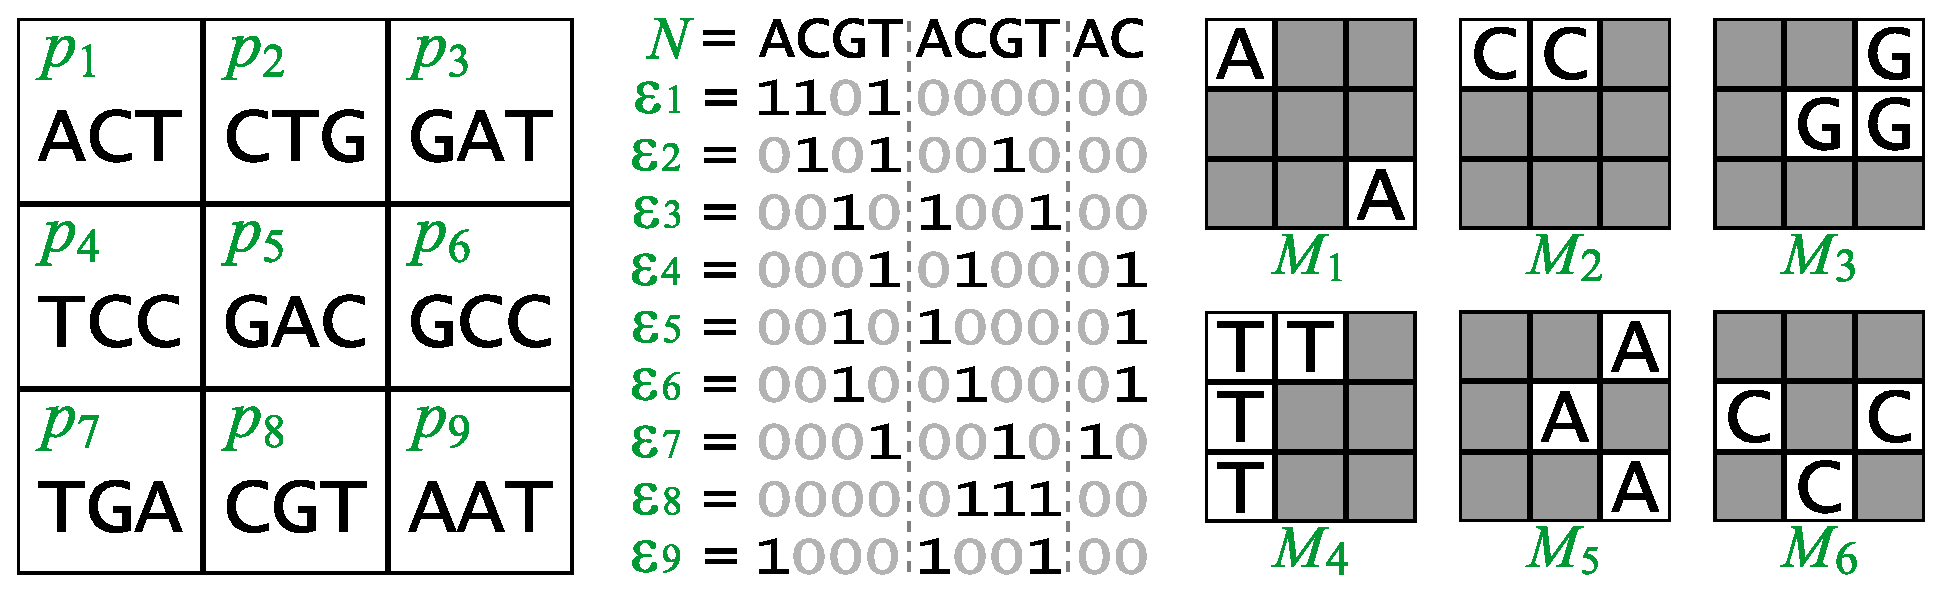
\includegraphics[width=\textwidth]{figures/chip.eps}}
\caption{Synthesis of a hypothetical 3$\times$3 chip with photolithographic
  masks. Left: chip layout and the 3-mer probe sequences. Center: deposition
  sequence with 2.5 cycles and probe embeddings (asynchronous). Right: first six
  masks.}
\label{fig:masking_process}
\end{figure}

The deposition sequence is often a repeated permutation of the alphabet, mainly
because of its regular structure and because such sequences maximize the number
of distinct subsequences \citep{Chase1976}. The deposition sequence shown in
Fig.~\ref{fig:masking_process} is a 2.5-time repetition of ACGT, and we thus say
that it has two and a half \emph{cycles}.

For cyclic deposition sequences, it is possible to distinguish between two types
of embeddings: \emph{synchronous} and \emph{asynchronous}. In the former, each
probe has exactly one nucleotide synthesized in every cycle of the deposition
sequence; hence, 25 cycles or 100 steps are needed to synthesize probes of
length 25. With asynchronous embeddings, probes can have any number of
nucleotides synthesized in any given cycle, allowing shorter deposition
sequences. For this reason, asynchronous embeddings are usually the choice for
commercial microarrays.  For instance, all GeneChip arrays that we know of can
be asynchronously synthesized in 74~steps with 18.5 cycles of TGCA --- we will
refer to this sequence as the \emph{standard Affymetrix deposition sequence}.

Ideally, the deposition sequence should be as short as possible in order to
reduce manufacturing time, cost and probability of errors \citep{Rahmann2003}.
Finding the shortest deposition sequence to synthesize a set of probes is an
instance of a classical computer science problem known as the Shortest Common
Supersequence problem, which will be the focus of Chapter~\ref{ch:scs}. For the
MLP, however, we assume that $N$ is a fixed sequence given as input.

%%%%%%%%%%%%%%%%%%%%%%%%%%%%%%%%%%%%%%%%%%%%%%%%%%%%%%%%%%%%%%%%%%%%%%%%%%%%%%%%
\section{Problem statement}
\label{sec:mlp_problem}

Given a set of probes $\CalP$, a geometry of spots $\CalS$, and a deposition
sequence $N$ as specified above, the MLP asks to specify a chip layout
$(k,\eps)$ that consists of
\begin{enumerate}
\item a bijective assignment $k: \CalS\to \{1,\dots,n\}$ that specifies a probe
  index $k(s)$ for each spot $s$ (meaning that $p_{k(s)}$ will be synthesized at
  $s$),
\item an assignment $\eps: \{1,\dots,n\}\to \{0,1\}^T$ specifying an embedding
  $\eps_k = (\eps_{k,1},\dots,\eps_{k,T})$ for each probe index $k$, such that
  $N[\eps_k] :\equiv (N_t)_{t: \eps_{k,t}=1} = p_k$,
\end{enumerate}
such that a given penalty function is minimized.  We introduce two such penalty
functions: total border length and total conflict index.

%We may thus speak of $\eps_{k(s)}$ as the embedding at spot $s$.

%%%%%%%%%%%%%%%%%%%%%%%%%%%%%%%%%%%%%%%%%%%%%%%%%%%%%%%%%%%%%%%%%%%%%%%%%%%%%%%%
\section{Border length}
\label{sec:mlp_border_length}

The first formal definition to the problem of unintended illumination was given
by \citet{Hannenhalli2002}, who defined the \emph{border length}~$\CalB_t$ of a
mask~$M_{t}$ as the number of borders separating masked and unmasked spots at
synthesis step~$t$, that is, the number of border conflicts in $M_{t}$.
Formally,
%%
\begin{equation}
\label{eq:border_length}
  \CalB_t := \frac{1}{2} \cdot \sum_{s,s' \in \CalS}
    \Ind{s \text{ and } s' \text{ are adjacent}}
    \cdot \Ind{\eps_{k(s),t} \neq \eps_{k(s'),t}}.
\end{equation}
%%
where $\Ind{cond}$ is the indicator function that equals 1 if condition $cond$
is true, and 0 otherwise. The total border length of a given layout $(k,\eps)$
is the sum of border lengths over all masks, that is
%%
\begin{equation}
\label{eq:total_border_length}
  \CalB(k,\eps) := \sum_{t=1}^{T} \CalB_t.
\end{equation}

The \emph{Border Length Minimization Problem} was then defined as the problem of
finding a layout minimizing the total border length \citep{Hannenhalli2002}. As
an example, the six masks shown in Fig.~\ref{fig:masking_process} have
$\CalB_1 = 4$, $\CalB_2 = 3$, $\CalB_3 = 5$, $\CalB_4 = 4$, $\CalB_5 = 8$ and
$\CalB_6 = 9$. The total border length of that layout is 52 (masks 7 to 10 not
shown).

\paragraph{Hamming distance.}
In the rest of this thesis, we will refer to the \emph{Hamming distance}
$H(k,k')$ between the embeddings $\eps_k$ and $\eps_{k'}$ as the number of
synthesis steps in which they differ. Formally,
%%
\begin{equation}
\label{eq:hamming}
  H(k,k') := \sum_{t=1}^{T} \Ind{\eps_{k,t} \neq \eps_{k',t}}.
\end{equation}

Note that $H(k,k')$ gives the number of border conflicts generated when probes
with embeddings $\eps_k$ and $\eps_{k'}$ are placed in adjacent spots.

\subsection{Lower Bounds}

Lower bounds for the BLMP with synchronous and asynchronous embeddings were
given by \citet{Kahng2002}, based on a simple graph formulation. Unfortunately,
both lower bounds are not tight, and their computation is time-consuming,
especially for large chips.

\paragraph{Synchronous embeddings.}
Let $L$ be a complete directed graph over the set of probes $\CalP$ with arcs
weighted with the Hamming distance between the (unique) embeddings of the
corresponding probes.

Since a probe can have at most four neighbors on the chip, we delete all but the
four arcs with the least weights of every node. Furthermore, assuming that the
chip is a rectangular grid with $n_r$ rows and $n_c$ columns, we delete the
heaviest $2 \cdot (n_r + n_c)$ remaining arcs, because the spots on the borders
of the chip have less than four neighbors. It is not difficult to see that the
cost of any placement must be greather than the total weight of $L$, and we
obtain the following theorem.

\begin{theorem}
  \label{thm:sync_lb}
  The total arc weight of $L$ is a lower bound on the total border length of
  the optimum layout with synchronous embeddings.
\end{theorem}

\paragraph{Asynchronous embeddings.}
With asynchronous embeddings, we can construct a similar complete directed graph
$L'$. For the arc weights, however, it is necessary to estimate the minimum
number of border conflicts between the two probes (among all of their possible
embeddings).

\citet{Kahng2002} observed that the number of bases of a probe $p_k$ that can
be ``aligned'' with bases of $p_{k'}$ cannot exceed the length of $LCS(p_k,p_{k'})$,
where $LCS(p_k,p_{k'})$ is the
\emph{longest common subsequence} of $p_k$ and $p_{k'}$. Therefore, an arc of $L'$
between probes $p_k$ and $p_{k'}$ can be weighted with $\ell - |LCS(p_k,p_{k'})|$,
where $\ell$ is the length of both probe sequences (assuming probes have the same length).

We can then delete all but the four arcs with the least weights of each probe
and, subsequently, the heaviest $2 \cdot (n_r + n_c)$ remaining arcs of $L'$, to
obtain the following theorem.

\begin{theorem}
  \label{thm:async_lb}
  The total arc weight of $L'$ is a lower bound on the total border length of
  the optimum layout with asynchronous embeddings.
\end{theorem}

%%%%%%%%%%%%%%%%%%%%%%%%%%%%%%%%%%%%%%%%%%%%%%%%%%%%%%%%%%%%%%%%%%%%%%%%%%%%%%%%
\section{Conflict index}
\label{sec:mlp_conflict_index}

The border length measures the quality of an individual mask or set of masks.
With this model, however, it is not possible to know how the border conflicts
are distributed among the probes. Ideally, all probes should have roughly the
same risk of being damaged by unintended illumination, so that all signals are
affected in approximately the same way.

The \emph{conflict index} is a quality measure defined with the aim of
estimating the risk of damaging probes at a particular spot
\citep{Carvalho2006a} -- it is thus a per-spot or per-probe measure instead of a
per-mask measure.  Additionally, it takes into account two practical
considerations observed by \citet{Kahng2003}:
%%
\begin{itemize}
\item[a)] stray light might activate not only adjacent neighbors but also spots
  that lie as far as three cells away from the targeted spot;
\item[b)] imperfections produced in the middle of a probe are more harmful than
  in its extremities.
\end{itemize}

For a proposed layout $(k,\eps)$, the conflict index~$\CalC(s)$ of a spot $s$
whose probe $p_{k(s)}$ is synthesized in $T$~masking steps according to its
embedding vector $\eps_{k(s)}$ is
%%
\begin{equation}
\label{eq:conf_idx}
\CalC(s) := \sum_{t=1}^{T} \Bigl(
  \Ind{\eps_{k(s),t}=0}
  \cdot \omega(\eps_{k(s)},t)
  \cdot \sum_{\substack{s'\text{: neighbor}\\\text{of } s}}
  \Ind{\eps_{k(s'),t}=1}
  \cdot \gamma(s,s') \Bigr).
\end{equation}

The indicator functions ensure the following conflict condition: During
step~$t$, there is a conflict at spot~$s$ if and only if $s$ is masked
($\eps_{k(s),t}=0$) and a close neighbor $s'$ is unmasked ($\eps_{k(s'),t}=1$),
since light directed at $s'$ may somehow reach $s$.  When $s$ is productive, it
does not matter if it accidentally receives light targeted at a neighbor, and
when $s'$ is unproductive, there is no risk that it damages probes of $s$.

Function $\gamma(s,s')$ is a ``closeness'' measure between $s$ and $s'$ (to
account for observation a). It is defined as
%%
\begin{equation}\label{eq:dist_weight}
\gamma(s,s') := (d(s,s'))^{-2},\nopagebreak
\end{equation}\nopagebreak
%%
where $d(s,s')$ is the Euclidean distance between the spots $s$ and $s'$. Note
that in (\ref{eq:conf_idx}), $s'$ ranges over all neighboring spots that are at
most three cells away from $s$ (see Fig.~\ref{fig:conflictindex}~left), which is
in accordance with observation a.

In general, we use the terms \emph{close neighbor} or simply \emph{neighbor} of
a spot $s$ to refer to a spot $s'$ that is at most three cells away (vertically
and horizontally) from $s$. In other words, $s'$ is inside a $7\times 7$ region
centered around $s$. This is in contrast to the terms \emph{direct} or \emph{
immediate neighbor} of $s$, used to denote a spot $s'$ that is adjacent to $s$
(in other words, $s'$ shares a common border with $s$ on the chip). Obviously,
an immediate neighbor $s'$ is also a close neighbor of $s$.

The position-dependent weighting function $\omega(\eps,t)$ accounts for the
significance of the location inside the probe where the undesired nucleotide is
introduced in case of accidental illumination (observation b). It is defined as:
%%
\begin{equation}\label{eq:pos_mult}
\omega(\eps,t) := c \cdot \exp{\left(\theta \cdot \lambda(\eps,t)\right)}
\end{equation}
%%
where $c>0$ and $\theta>0$ are constants, and for $1\leq t\leq T$,
%%
\begin{equation}\label{eq:base_pos}
  \lambda(\eps,t) := 1 + \min(b_{\eps,t},\ell_{\eps} - b_{\eps,t}),
\end{equation}
%%
\begin{equation}\label{eq:b_ell}
  b_{\eps,t} := \sum_{t'=1}^{t} \eps_{t'},
  \qquad
  \ell_{\eps} := \sum_{t=1}^{T} \eps_t = b_{\eps,T}.
\end{equation}

In other words, $\ell_\eps$ is the length of the final probe specified by $\eps$
(equal to the number of ones in the embedding), and $b_{\eps,t}$ denotes the
number of nucleotides synthesized up to and including step~$t$.

Note that $\omega(\eps,t)$ grows exponentially from the extremities of the probe
to its center (see Fig.~\ref{fig:conflictindex} right). The motivation behind
this definition is that the probability of a successful stable hybridization of
a probe with its target should increase exponentially with the absolute value of
its Gibbs free energy, which increases linearly with the length of the longest
perfect match between probe and target. The parameter $\theta$ controls how
steeply the exponential weighting function rises towards the middle of the
probe. In Fig.~\ref{fig:conflictindex} and our experiments, we use probes of
length $\ell=25$, and parameters $\theta = 5/\ell$ and $c = 1/\exp{(\theta)}$.

Although it is generally agreed that the chances of a successful hybridization
between probe and target are higher if a mismatched base occurs at the
extremities of the formed duplex instead of at its center \citep{Hubbell1999}.
The precise effects of this position is not yet fully understood and has been an
active topic of research \citep{Binder2005}.

\begin{figure}
%%
\begin{picture}(180,140)
  \put(0,0){\makebox(180,140){
    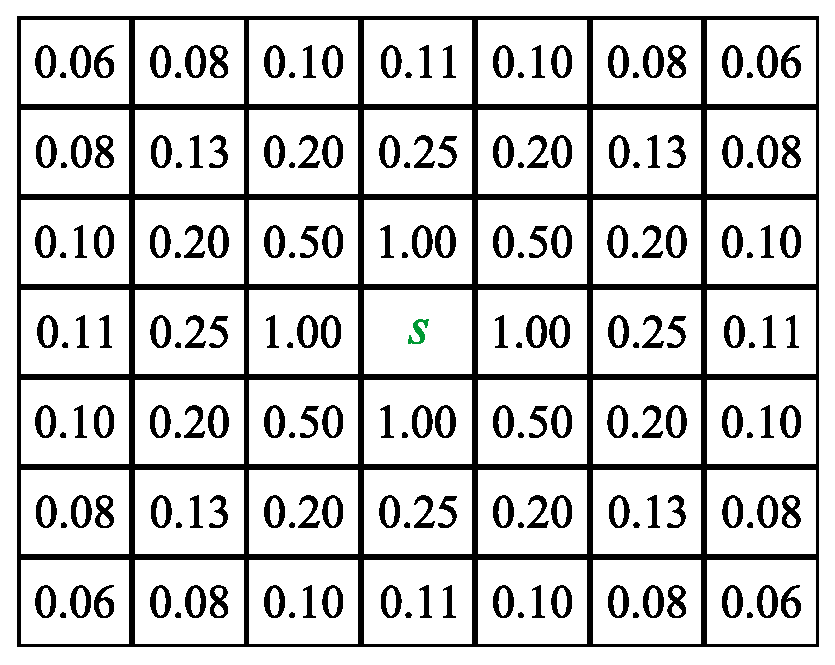
\includegraphics[width=0.4\textwidth]{distweights}
  }}
\end{picture}
%%
\begin{picture}(255,140)
  \footnotesize{
    \put(0,0){\makebox(255,140){
      %GNUPLOT: LaTeX picture with Postscript
      \begin{picture}(0,0)%
      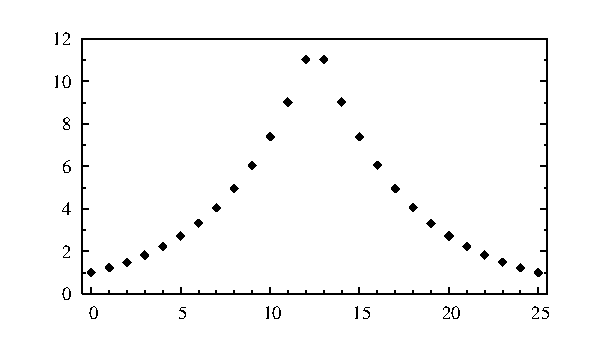
\includegraphics{posweights}%
      \end{picture}%
      \begingroup
      \setlength{\unitlength}{0.0200bp}%
      \begin{picture}(13500,7019)(0,0)%
      \put(1250,1000){\makebox(0,0)[r]{\strut{} 0}}%
      \put(1250,1920){\makebox(0,0)[r]{\strut{} 2}}%
      \put(1250,2840){\makebox(0,0)[r]{\strut{} 4}}%
      \put(1250,3760){\makebox(0,0)[r]{\strut{} 6}}%
      \put(1250,4680){\makebox(0,0)[r]{\strut{} 8}}%
      \put(1250,5600){\makebox(0,0)[r]{\strut{} 10}}%
      \put(1250,6520){\makebox(0,0)[r]{\strut{} 12}}%
      \put(1716,500){\makebox(0,0){\strut{} 0}}%
      \put(3880,500){\makebox(0,0){\strut{} 5}}%
      \put(6043,500){\makebox(0,0){\strut{} 10}}%
      \put(8207,500){\makebox(0,0){\strut{} 15}}%
      \put(10370,500){\makebox(0,0){\strut{} 20}}%
      \put(12534,500){\makebox(0,0){\strut{} 25}}%
      \end{picture}%
      \endgroup
    }}
  }
\end{picture}
%%
\vspace*{-3ex}
\caption{\label{fig:conflictindex}
  Ranges of values for both $\gamma$ and $\omega$ on a typical Affymetrix
  chip where probes of length~25 are synthesized in~74 masking steps. Left:
  approximate values of the distance-dependent weighting function
  $\gamma(s,s')$ for a spot $s$ in the center and close
  neighbors~$s'$. Right:
  position-dependent weights $\omega(\eps,t)$ on the y-axis for each value
  of~$b_{\eps,t}\in\{0,\dots,25\}$ on the x-axis, assuming $\ell_\eps=25$.}%
\end{figure}

\paragraph{Conflict Index distance.}
Many of the algorithms that will be discussed in later chapters were initially
developed for border length minimization, and they usually rely on the Hamming
distance defined earlier (\ref{eq:hamming}). We have adapted some of these
algorithms to work with conflict index minimization by using the \emph{conflict
index distance}, which extends the Hamming distance by taking into account the
position inside the probe where the conflict occurs (observation b). We define
the conflict index distance $C(k,k')$ between the embeddings $\eps_k$ and
$\eps_{k'}$ as:
%%
\begin{equation}
\label{eq:ci_dist}
C(k,k') := \sum_{t=1}^{T}
  \Bigl(
    \Ind{\eps_{k,t}=0 \text{ and } \eps_{k',t}=1}
    \cdot \omega(\eps_{k},t)
    +
    \Ind{\eps_{k',t}=0 \text{ and } \eps_{k,t}=1}
    \cdot \omega(\eps_{k'},t)
  \Bigr).
\end{equation}

The conflict index distance $C(k,k')$ can be interpreted as the sum of the
conflict indices resulting from placing probes $p_k$ and $p_{k'}$ at
hypothetical neighboring spots, ignoring the distance between these spots (note
that there is no dependency on $\gamma$) and the conflicts generated by other
neighbors.

\subsection{The Meaning of Conflict Index}

The conflict index $\CalC(s)$ attempts to estimate the risk of damaging the
probes of a spot $s$ due to the unwanted illumination problem. The definitions
of $\gamma$ and $\omega$ given here are an arbitrary choice in an attempt to
capture the characteristics of the problem.

The most appropriate choice of $\gamma$ and $\omega$ depend on several
attributes of the specific technology used to produce the chips such as the
physical properties of the light (intensity, frequency, etc.), the size of the
spots, the density of the probes on the chip, the distance between the light
source and the mask and the distance between the mask and the chip surface.

Finding the best choice of $\gamma$ and $\omega$ for a particular technology is
beyond the scope of this thesis. We note, however, that all algorithms discussed
in the next chapters were developed to work independently of the values given by
these functions.

%%%%%%%%%%%%%%%%%%%%%%%%%%%%%%%%%%%%%%%%%%%%%%%%%%%%%%%%%%%%%%%%%%%%%%%%%%%%%%%%
\section{Chip Quality Measures}
\label{sec:mlp_bl_vs_ci}

Most of the algorithms discussed in the next chapters can work with border
length as well as conflict index minimization. The relation between these two
measures becomes clear if $\gamma(s,s')$ and $\omega(\eps,t)$ are re-defined as
follows: Set $\gamma(s,s') := 1$ if $s'$ is a direct neighbor of~ $s$, and $:=0$
otherwise. Also, set $\omega(\eps,t) := 1/2$, so that conflicts always have the
same weight, independently of where they occur. Now
$\sum_s\, \CalC(s) = \sum_{t=1}^T\, \CalB_t$; that is, total border length is
equivalent to the sum of conflict indices for a particular choice of $\gamma$
and $\omega$. For the choices~(\ref{eq:dist_weight}) and~(\ref{eq:pos_mult}),
they are not equivalent but still correlated, since a good layout has low border
lengths as well as low conflict indices.

To better compare border lengths for chips of different sizes, we divide by the
number of internal borders of the chip $n_b$, which equals
$n_b = n_r(n_c - 1) + n_c(n_r - 1)$, assuming that the chip is a rectangular
grid with $n_r$ rows and $n_c$ columns. We thus call
$1/n_b \cdot \sum_{t=1}^T\, \CalB_t$ the \emph{normalized border length}. This
can be further divided by the number of synthesis steps to give the
\emph{normalized border length per mask}
$1/(n_b \cdot T) \cdot \sum_{t=1}^T\, \CalB_t$.

Similarly, it is useful to divide the total conflict index by the number of
probes, and we define the \emph{average conflict index} as
$1/|\CalP| \cdot \sum_s\, \CalC(s)$.

%%%%%%%%%%%%%%%%%%%%%%%%%%%%%%%%%%%%%%%%%%%%%%%%%%%%%%%%%%%%%%%%%%%%%%%%%%%%%%%%
\section{How hard is the Microarray Layout Problem?}
\label{sec:mlp_how_hard}

The MLP appears to be hard because of the super-exponential number of possible
arrangements, although no NP-hardness proof is yet known. A formulation of the
MLP as a Quadratic Assignment Problem (QAP) was given by \citet{Carvalho2006a}.
The QAP is a classical combinatorial optimization problem that is, in general,
NP-hard, and particularly hard to solve in practice \citep{Cela1997}. Optimal
solutions are thus unlikely to be found even for small chips and even if we
assume that all probes have a single predefined embedding.

If we consider all possible embeddings (up to several million for a typical
Affymetrix probe), the MLP is even harder. For this reason, the problem has been
traditionally tackled in two phases. First, an initial embedding of the probes
is fixed and an arrangement of these embeddings on the chip with minimum
conflicts is sought. This is usually referred to as the \emph{placement} phase.
Second, a post-placement optimization phase \emph{re-embeds} the probes
considering their location on the chip, in such a way that the conflicts with
neighboring spots are further reduced. Often, the chip is \emph{partitioned}
into smaller sub-regions before the placement phase in order to reduce running
times, especially on larger chips.

The most important placement algorithms are surveyed in
Chapter~\ref{ch:placement}. The QAP formulation of the MLP is then presented in
Chapter~\ref{ch:qap}. Re-embedding algorithms are discussed in
Chapter~\ref{ch:reembed}, whereas partitioning algorithms are the focus of
Chapter~\ref{ch:part}. Finally, we present recent developments that
simultaneously place and re-embed probes in Chapter~\ref{ch:merge}.
